% This file was converted to LaTeX by Writer2LaTeX ver. 1.4
% see http://writer2latex.sourceforge.net for more info
\documentclass[letterpaper]{article}
\usepackage[latin1]{inputenc}
\usepackage[T1]{fontenc}
\usepackage[english]{babel}
\usepackage{amsmath}
\usepackage{amssymb,amsfonts,textcomp}
\usepackage{color}
\usepackage[top=2cm,bottom=2cm,left=2cm,right=2cm,nohead,nofoot]{geometry}
\usepackage{array}
\usepackage{supertabular}
\usepackage{hhline}
\usepackage{hyperref}
\hypersetup{colorlinks=true, linkcolor=blue, citecolor=blue, filecolor=blue, urlcolor=blue, pdftitle=}
\usepackage[pdftex]{graphicx}
\makeatletter
\newcommand\arraybslash{\let\\\@arraycr}
\makeatother
% Footnote rule
\setlength{\skip\footins}{0.119cm}
\renewcommand\footnoterule{\vspace*{-0.018cm}\setlength\leftskip{0pt}\setlength\rightskip{0pt plus 1fil}\noindent\textcolor{black}{\rule{0.25\columnwidth}{0.018cm}}\vspace*{0.101cm}}
\setlength\tabcolsep{1mm}
\renewcommand\arraystretch{1.3}
\title{}
\begin{document}
\section[Audacity Tour Guide]{\textmd{\textcolor{black}{Audacity Tour Guide}}}
{\color{black}
This guide provides a quick tour of selected features of Audacity. This page doesn't tell you how to use features, it
would be much too long if it did. Rather it tells you about some of the features that exist in Audacity and will help
you learn a little about those.}

{\color{black}
There are many links on this page (highlighted in blue). Click the links to go to the more detailed pages in the
Manual.}

\textcolor{black}{Also remember that
the~}\href{https://manual.audacityteam.org/index.html#reference}{\textbf{\textcolor[rgb]{0.3529412,0.21176471,0.5882353}{Screenshot
of Audacity}}}\textcolor{black}{~on the front page is clickable. Clicking on a feature will take you to the place in
the Manual that describes that feature.}

\subsection[Record, Play and Edit {}- the basics of Audacity]{\color{black} Record, Play and Edit - the basics of
Audacity}
\textcolor{black}{Audacity
can~}\href{https://manual.audacityteam.org/man/playback.html}{\textbf{\textcolor[rgb]{0.3529412,0.21176471,0.5882353}{Play}}}\textcolor{black}{~}

\includegraphics[width=0.423cm,height=0.423cm]{TourGuide-img001.png}
\textcolor{black}{~}\href{https://manual.audacityteam.org/man/recording.html}{\textbf{\textcolor[rgb]{0.3529412,0.21176471,0.5882353}{Record}}}\textcolor{black}{~}

\includegraphics[width=0.423cm,height=0.423cm]{TourGuide-img002.png}
\textcolor{black}{~and~}\href{https://manual.audacityteam.org/man/edit.html}{\textbf{\textcolor[rgb]{0.3529412,0.21176471,0.5882353}{edit}}}\textcolor{black}{~audio.
To play or record, click on the button on the toolbar:}

 
\includegraphics[width=8.652cm,height=1.455cm]{TourGuide-img003.png} 

Transport Toolbar Play~ 
\includegraphics[width=0.423cm,height=0.423cm]{TourGuide-img001.png} ~and Record~

\includegraphics[width=0.423cm,height=0.423cm]{TourGuide-img002.png} ~buttons

{\color{black}
~\\
\newline
Hold~\textbf{\textit{Shift}}~down, and those two buttons change to~\textbf{Loop Play}~

\includegraphics[width=0.423cm,height=0.423cm]{TourGuide-img004.png} ~and~\textbf{Record New Track}~

\includegraphics[width=0.423cm,height=0.423cm]{TourGuide-img005.png} .}

 
\includegraphics[width=8.652cm,height=1.455cm]{TourGuide-img006.png} 

Transport Toolbar with~Shift~held down

\subsubsection[Loop
Play]{\href{https://manual.audacityteam.org/man/playing_and_recording.html\#transport}{\textcolor[rgb]{0.3529412,0.21176471,0.5882353}{Loop
Play}}}
{\color{black}
Hold~\textbf{\textit{Shift}}~and the play button will change from~

\includegraphics[width=0.423cm,height=0.423cm]{TourGuide-img001.png} ~to~

\includegraphics[width=0.423cm,height=0.423cm]{TourGuide-img004.png} ~the Loop Play button. Click on this and you will
get Loop Play where the audio plays over and over until you stop.}

\subsubsection[New Track
Record]{\href{https://manual.audacityteam.org/man/recording.html\#newtrack}{\textcolor[rgb]{0.3529412,0.21176471,0.5882353}{New
Track Record}}}
{\color{black}
Hold~\textbf{\textit{Shift}}~and the record button changes from~

\includegraphics[width=0.423cm,height=0.423cm]{TourGuide-img002.png} ~to~

\includegraphics[width=0.397cm,height=0.397cm]{TourGuide-img005.png} ~\textbf{\textit{Record New Track}}.
Click,~\textit{(or use shortcut~}\textbf{\textit{Shift + R}}\textit{~)}~to start recording in a new track at either the
current cursor position or at the beginning of the current selection.}

{\color{black}
By default Audacity will record at the end of the currently selected (or only) track}

\subsubsection[Select and
Edit]{\href{https://manual.audacityteam.org/man/selecting_audio_the_basics.html}{\textcolor[rgb]{0.3529412,0.21176471,0.5882353}{Select
and Edit}}}
\href{https://manual.audacityteam.org/man/selecting_audio_the_basics.html}{\textcolor[rgb]{0.3529412,0.21176471,0.5882353}{Select}}\textcolor{black}{~audio
by dragging, before using buttons
like~}\href{https://manual.audacityteam.org/man/edit_toolbar.html}{\textcolor[rgb]{0.3529412,0.21176471,0.5882353}{cut,
copy and paste}}\textcolor{black}{~to rearrange the audio. You can also apply
an~}\href{https://manual.audacityteam.org/man/effect_menu_audacity.html}{\textcolor[rgb]{0.3529412,0.21176471,0.5882353}{audio
effect}}\textcolor{black}{~to the selected audio.}

 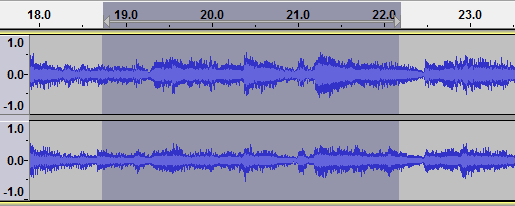
\includegraphics[width=13.626cm,height=5.45cm]{TourGuide-img007.png} 

Example of a stereo audio track with some audio selected - the selection is the dark gray section

\textcolor{black}{For more details on Play, Record and Edit see
the~}\href{https://manual.audacityteam.org/quick_help.html}{\textcolor[rgb]{0.3529412,0.21176471,0.5882353}{Getting
Started}}\textcolor{black}{~section of the Manual.}

\subsection[Saving your work {}- audio formats]{\color{black} Saving your work - audio formats}
\subsubsection[Save]{\href{https://manual.audacityteam.org/man/file_menu.html\#save}{\textcolor[rgb]{0.3529412,0.21176471,0.5882353}{Save}}}
\textcolor{black}{Audacity makes a distinction between saving audio
in~}\href{https://manual.audacityteam.org/man/audacity_projects.html}{\textbf{\textcolor[rgb]{0.3529412,0.21176471,0.5882353}{Audacity
project format}}}\textcolor{black}{~which only Audacity can open, and exporting audio in formats like WAV and MP3 for
use in other applications. Audacity project format is made up of multiple small files which are stored in the \_data
folder for the project and alongside that, an AUP file which says what order the files are in. To reopen a saved
project, open the AUP file,~}\textbf{\textit{\textcolor{black}{not}}}\textcolor{black}{~the multiple small files.}

\subsubsection[Export]{\href{https://manual.audacityteam.org/man/file_export_dialog.html}{\textcolor[rgb]{0.3529412,0.21176471,0.5882353}{Export}}}
{\color{black}
Use Export if you want to create a file in an audio format for playing outside of Audacity.}

\begin{itemize}
\item
\href{https://manual.audacityteam.org/man/faq_installation_and_plug_ins.html#lame}{\textbf{\textcolor[rgb]{0.3529412,0.21176471,0.5882353}{LAME}}}\textbf{\textcolor{black}{:}}\textcolor{black}{~Do
you want to convert a recording to compressed MP3 format? Audacity can, but it needs an add-on to do so. The add-on is
a library called `LAME'. A free copy of LAME that is compatible with Audacity is available from the lame.buanzo.org
site, as
per~}\href{https://manual.audacityteam.org/man/faq_installation_and_plug_ins.html#lame}{\textcolor[rgb]{0.3529412,0.21176471,0.5882353}{these
instructions}}\textcolor{black}{~(Buanzo is a technology and security consultant from Argentina).}
\item
\href{https://manual.audacityteam.org/man/faq_installation_and_plug_ins.html#ffdown}{\textbf{\textcolor[rgb]{0.3529412,0.21176471,0.5882353}{FFmpeg}}}\textbf{\textcolor{black}{:}}\textcolor{black}{~The
optional~}\href{https://manual.audacityteam.org/man/faq_opening_and_saving_files.html#foreign}{\textcolor[rgb]{0.3529412,0.21176471,0.5882353}{FFmpeg
library}}\textcolor{black}{~allows Audacity to import and export a much
larger~}\href{https://wiki.audacityteam.org/wiki/FFmpeg_integration#Functionality}{\textit{\textcolor[rgb]{0.2,0.4,0.73333335}{range
of audio
formats}}}\textcolor{black}{~including~}\href{https://manual.audacityteam.org/man/glossary.html#aac}{\textbf{\textit{\textcolor[rgb]{0.3529412,0.21176471,0.5882353}{M4A
(AAC)}}}}\textcolor{black}{, AC3, AMR (narrow band)
and~}\href{https://manual.audacityteam.org/man/glossary.html#wma}{\textbf{\textit{\textcolor[rgb]{0.3529412,0.21176471,0.5882353}{WMA}}}}\textcolor{black}{.
Audacity can import audio from most video files by using FFmpeg.}
\end{itemize}
\subsection[Themes]{\href{https://manual.audacityteam.org/man/themes.html}{\textmd{\textcolor[rgb]{0.3529412,0.21176471,0.5882353}{Themes}}}}
\textcolor{black}{Audacity has four pre-configured, user-selectable, themes. This enables you to choose the look and
feel you prefer for Audacity's interface. see
the~}\href{https://manual.audacityteam.org/man/themes.html}{\textcolor[rgb]{0.3529412,0.21176471,0.5882353}{Themes}}\textcolor{black}{~page
for details.}

\begin{itemize}
\item {\color{black}
\textbf{Light}~theme: this is a light theme loosely based on the look and feel of earlier Audacity versions, but given a
contemporary twist with more modern-looking buttons and icons.}
\item \textbf{\textcolor{black}{Dark}}\textcolor{black}{~theme: created by
the~}\href{http://www.darkaudacity.com/}{\textit{\textcolor[rgb]{0.2,0.4,0.73333335}{Dark Audacity
project.}}}\textcolor{black}{~This is similar to the Light theme, with the same buttons and icons, but given a dark
twist.}
\item {\color{black}
\textbf{Classic}~theme: The one you know and loved. This theme is a re-creation of the look and feel of earlier Audacity
versions.}
\item {\color{black}
\textbf{High Contrast}~theme: some users with poor eyesight benefit from a high contrast that is 'eye-popping' for most
people.}
\end{itemize}
\begin{flushleft}
\tablefirsthead{}
\tablehead{}
\tabletail{}
\tablelasttail{}
\begin{supertabular}{m{0.40100002cm}m{10.588cm}m{0.375cm}m{10.667cm}}
~~~~ &
\href{https://manual.audacityteam.org/man/themes.html#light}{
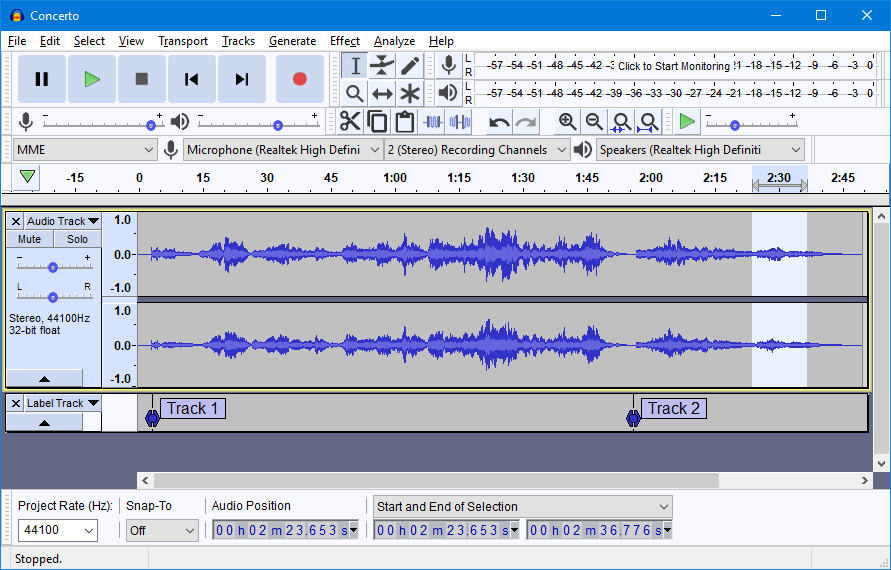
\includegraphics[width=10.636cm,height=6.826cm]{TourGuide-img008.png} } &
~~~~ &
\href{https://manual.audacityteam.org/man/themes.html#dark}{
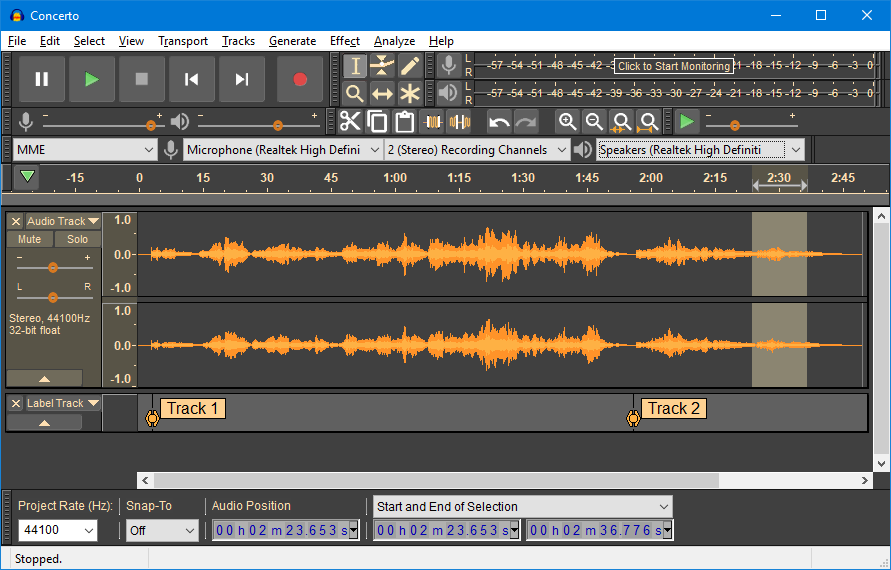
\includegraphics[width=10.636cm,height=6.826cm]{TourGuide-img009.png} }\\
~~~~ &
\centering \textbf{Light}~theme &
~~~~ &
\centering\arraybslash \textbf{Dark}~theme\\
\end{supertabular}
\end{flushleft}
\begin{flushleft}
\tablefirsthead{}
\tablehead{}
\tabletail{}
\tablelasttail{}
\begin{supertabular}{m{0.40100002cm}m{10.588cm}m{0.375cm}m{10.667cm}}
~~~~ &
\href{https://manual.audacityteam.org/man/themes.html#classic}{
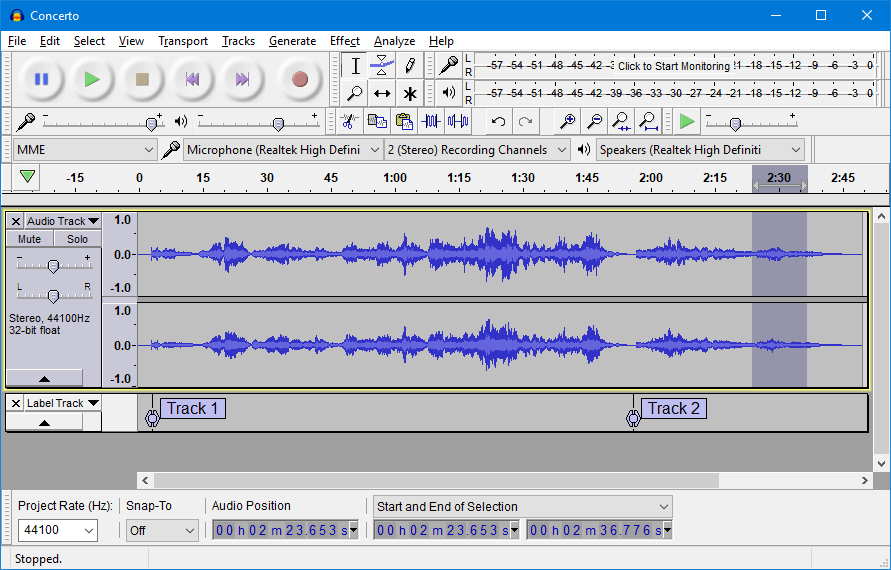
\includegraphics[width=10.636cm,height=6.826cm]{TourGuide-img010.png} } &
~~~~ &
\href{https://manual.audacityteam.org/man/themes.html#hicontrast}{
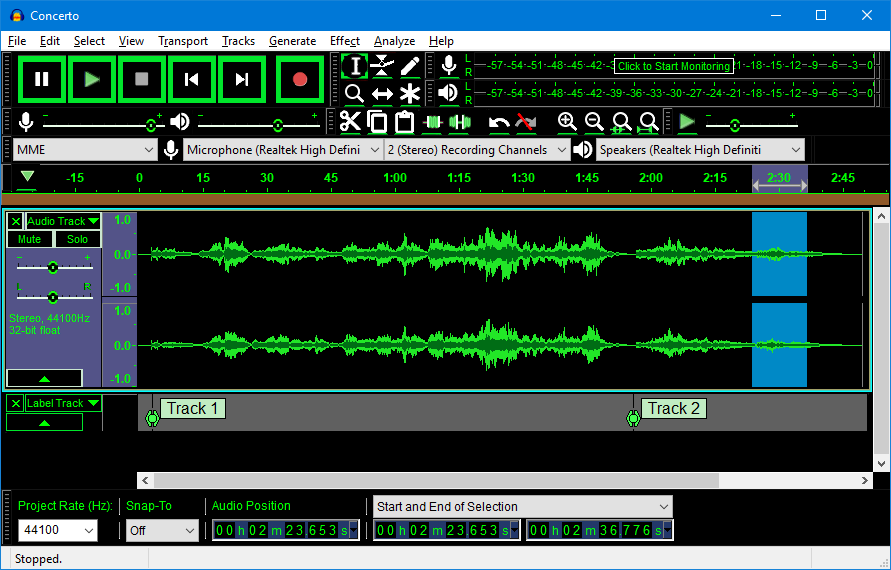
\includegraphics[width=10.636cm,height=6.826cm]{TourGuide-img011.png} }\\
~~~~ &
\centering \textbf{Classic}~theme &
~~~~ &
\centering\arraybslash \textbf{High Contrast}~theme\\
\end{supertabular}
\end{flushleft}
\subsection[Faster ways to do things {}- shortcuts and Chains]{\color{black} Faster ways to do things - shortcuts and
Chains}
 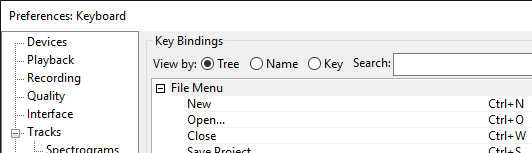
\includegraphics[width=14.076cm,height=4.048cm]{TourGuide-img012.png} 

A fragment of the keyboard preferences dialog showing some shortcuts

\subsubsection[Shortcuts]{\href{https://manual.audacityteam.org/man/keyboard_shortcut_reference.html}{\textcolor[rgb]{0.3529412,0.21176471,0.5882353}{Shortcuts}}}
\textcolor{black}{Many buttons and menu commands have
pre-defined~}\href{https://manual.audacityteam.org/man/keyboard_shortcut_reference.html}{\textcolor[rgb]{0.3529412,0.21176471,0.5882353}{keyboard
shortcuts}}\textcolor{black}{~assigned. You can modify these or add your own
with~}\href{https://manual.audacityteam.org/man/keyboard_preferences.html}{\textcolor[rgb]{0.3529412,0.21176471,0.5882353}{Keyboard
Preferences}}\textcolor{black}{~(in the Edit menu on Windows and Linux or the {\textquotedbl}Audacity{\textquotedbl}
menu on Mac).}

\subsubsection[Chains]{\href{https://manual.audacityteam.org/man/chains_for_batch_processing_and_effects_automation.html}{\textcolor[rgb]{0.3529412,0.21176471,0.5882353}{Chains}}}
\textcolor{black}{Ever want to do the same thing to a large number of audio files, for example remove noise from them
and convert to MP3? Chains is the feature for this. Give it a list of files to work through and tell it what sequence
of things to do. Programmers may want instead to
use~}\href{https://manual.audacityteam.org/man/scripting.html}{\textcolor[rgb]{0.3529412,0.21176471,0.5882353}{Scripting}}\textcolor{black}{,
an experimental but more flexible version of Chains. This needs a free experimental module called mod-script-pipe and
experience in programming.}

\subsubsection[Export
Multiple]{\href{https://manual.audacityteam.org/man/export_multiple.html}{\textcolor[rgb]{0.3529412,0.21176471,0.5882353}{Export
Multiple}}}
{\color{black}
You can save several audio files at once, rather than saving them one by one.}

\subsection[Changing the loudness of your audio {}- fades, Amplify, pan and gain]{\color{black} Changing the loudness of
your audio - fades, Amplify, pan and gain}
 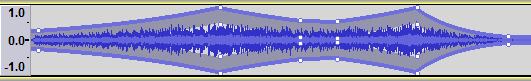
\includegraphics[width=14.049cm,height=2.143cm]{TourGuide-img013.png} 

Mono track showing an amplitude Envelope

\subsubsection[Amplify]{\href{https://manual.audacityteam.org/man/amplify.html}{\textcolor[rgb]{0.3529412,0.21176471,0.5882353}{Amplify}}}
\textcolor{black}{The~}\href{https://manual.audacityteam.org/man/amplify.html}{\textbf{\textcolor[rgb]{0.3529412,0.21176471,0.5882353}{Amplify}}}\textcolor{black}{~audio
effect makes audio louder or quieter. Two other effects that modify loudness
are~}\href{https://manual.audacityteam.org/man/fades.html#linearfade}{\textbf{\textcolor[rgb]{0.3529412,0.21176471,0.5882353}{Fade
In}}}\textcolor{black}{~and~}\href{https://manual.audacityteam.org/man/fades.html#linearfade}{\textbf{\textcolor[rgb]{0.3529412,0.21176471,0.5882353}{Fade
Out}}}\textcolor{black}{. These are often used at the beginning and end of audio.}

\begin{itemize}
\item
\href{https://manual.audacityteam.org/man/envelope_tool.html}{\textbf{\textcolor[rgb]{0.3529412,0.21176471,0.5882353}{Envelopes}}}\textcolor{black}{~provide
a more flexible way to control loudness. You will need to select
the~}\href{https://manual.audacityteam.org/man/envelope_tool.html}{\textbf{\textcolor[rgb]{0.3529412,0.21176471,0.5882353}{Envelope
Tool}}}\textcolor{black}{~or~}\href{https://manual.audacityteam.org/man/multi_tool.html}{\textbf{\textcolor[rgb]{0.3529412,0.21176471,0.5882353}{Multi-Tool}}}\textcolor{black}{~to
use envelopes. With envelopes you can graphically control when audio gets louder and quieter.}
\end{itemize}
\subsubsection[Pan~and~Gain]{\href{https://manual.audacityteam.org/man/audio_tracks.html\#pan}{\textcolor[rgb]{0.3529412,0.21176471,0.5882353}{Pan}}\textcolor{black}{~and~}\href{https://manual.audacityteam.org/man/audio_tracks.html\#gain}{\textcolor[rgb]{0.3529412,0.21176471,0.5882353}{Gain}}}
\textcolor{black}{These are the two sliders in the
track's~}\href{https://manual.audacityteam.org/man/audio_tracks.html#panel}{\textcolor[rgb]{0.3529412,0.21176471,0.5882353}{Track
Control Panel}}\textcolor{black}{. The~}\textbf{\textcolor{black}{Gain}}\textcolor{black}{~slider enables you to set
the loudness for the track. The~}\textbf{\textcolor{black}{Pan}}\textcolor{black}{~slider lets you make the audio
louder on the left or the right. You can move these sliders to affect the audio as it plays.}

\subsubsection[Mute~and~Solo]{\href{https://manual.audacityteam.org/man/audio_tracks.html\#mute}{\textcolor[rgb]{0.3529412,0.21176471,0.5882353}{Mute}}\textcolor{black}{~and~}\href{https://manual.audacityteam.org/man/audio_tracks.html\#solo}{\textcolor[rgb]{0.3529412,0.21176471,0.5882353}{Solo}}}
{\color{black}
These two buttons are in the track's Track Control Panel. Click the~Mute~button to silence this track when playing,
click again to hear it again. Click the~Solo~button to play just this track. Click again to release the button.}

\subsubsection[Auto
Duck]{\href{https://manual.audacityteam.org/man/auto_duck.html}{\textcolor[rgb]{0.3529412,0.21176471,0.5882353}{Auto
Duck}}}
\textcolor{black}{This reduces
(}\href{https://en.wikipedia.org/wiki/Ducking}{\textit{\textcolor[rgb]{0.2,0.4,0.73333335}{ducks}}}\textcolor{black}{)
the volume of one or more selected tracks whenever the volume of a single unselected {\textquotedbl}control
track{\textquotedbl} placed underneath reaches a particular threshold level. It can be used to create voice-overs for
podcasts or DJ sets, for automatic {\textquotedbl}ramping{\textquotedbl} of background music in radio productions and
for turning down a voice in original language as soon as its translation kicks in.}

\subsubsection[Mixer
Board]{\href{https://manual.audacityteam.org/man/mixer_board.html}{\textcolor[rgb]{0.3529412,0.21176471,0.5882353}{Mixer
Board}}}
{\color{black}
An alternative view to the audio tracks in the main tracks window, and is analogous to a hardware mixer board. Each
audio track is displayed in a Track Strip with its own pair of meters, gain slider, pan slider, and mute/solo buttons,
mirroring that track's controls in its Track Control Panel.}

\subsection[Noise in your audio {}- reducing, adding, fine tuning]{\color{black} Noise in your audio - reducing, adding,
fine tuning}
 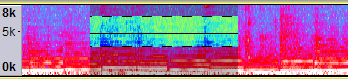
\includegraphics[width=9.208cm,height=2.09cm]{TourGuide-img014.png} 

Mono track in Spectrogram view showing a Spectral Selection

\subsubsection[Spectral
Selection]{\href{https://manual.audacityteam.org/man/spectral_selection.html}{\textcolor[rgb]{0.3529412,0.21176471,0.5882353}{Spectral
Selection}}}
\textcolor{black}{This is a special feature
within~}\href{https://manual.audacityteam.org/man/spectrogram_view.html}{\textbf{\textcolor[rgb]{0.3529412,0.21176471,0.5882353}{Sectrograms}}}\textcolor{black}{,
which lets you view the frequency content of audio then edit just selected frequencies. This is particularly useful for
voice recordings. Among other purposes, Spectral Selection and editing can be used for cleaning up unwanted sound by
removing particular frequencies, enhancing certain resonances, changing the quality of a voice or removing mouth sounds
from voice work.}

\subsubsection[Noise
Reduction]{\href{https://manual.audacityteam.org/man/noise_reduction.html}{\textcolor[rgb]{0.3529412,0.21176471,0.5882353}{Noise
Reduction}}}
{\color{black}
Audacity can remove some kinds of noise from a recording. Noise Reduction is an `audio effect', one of the fiddlier
audio effects to use. This effect works best with fairly constant noise like background hiss. You first select audio
that is just the noise and create a `noise profile'. Once Audacity knows the noise profile, it can reduce the loudness
of noise of that kind in audio you select.}

\subsubsection[Notch
Filter]{\href{https://manual.audacityteam.org/man/notch_filter.html}{\textcolor[rgb]{0.3529412,0.21176471,0.5882353}{Notch
Filter}}}
{\color{black}
This can be used to help you remove mains hum or electrical whistle with minimal damage to the remaining audio, by
cutting a {\textquotedbl}notch{\textquotedbl} out of the frequency spectrum at that point.}

\subsubsection[Generate
Noise]{\href{https://manual.audacityteam.org/man/generate_menu.html\#noise}{\textcolor[rgb]{0.3529412,0.21176471,0.5882353}{Generate
Noise}}}
{\color{black}
Audacity can add noise to a recording too. Three different types of noise can be generated. White noise has the greatest
ability to mask other sounds, as it has similar energy at all frequency levels. If you want to add some room noise to
make silences more realistic, try adding it at 0.001 amplitude.}

\subsubsection[Draw
Tool]{\href{https://manual.audacityteam.org/man/draw_tool.html}{\textcolor[rgb]{0.3529412,0.21176471,0.5882353}{Draw
Tool}}}
\textcolor{black}{If
you~}\href{https://manual.audacityteam.org/man/zooming.html}{\textbf{\textcolor[rgb]{0.3529412,0.21176471,0.5882353}{Zoom}}}\textcolor{black}{~in
enough on the audio you can edit individual samples of audio. Usually there are 44100 sample dots for every second of
audio. This gives you an idea of how the audio is stored in the computer. Very occasionally there may be a click in the
audio which is better removed with Draw Tool than
with~}\href{https://manual.audacityteam.org/man/click_removal.html}{\textbf{\textcolor[rgb]{0.3529412,0.21176471,0.5882353}{Click
Removal}}}\textcolor{black}{~or
the~}\href{https://manual.audacityteam.org/man/repair.html}{\textbf{\textcolor[rgb]{0.3529412,0.21176471,0.5882353}{Repair}}}\textcolor{black}{~effect.
Repair is best used when zoomed in a lot as it only works with short pieces of audio.}

\subsection[Navigation and changing speed and pitch]{\color{black} Navigation and changing speed and pitch}
\href{https://manual.audacityteam.org/man/toolbars_overview.html#upper_tooldock}{

\includegraphics[width=3.81cm,height=0.82cm]{TourGuide-img015.png} }

Transcription Toolbar

\subsubsection[Play{}-at{}-speed]{\href{https://manual.audacityteam.org/man/transcription_toolbar.html}{\textcolor[rgb]{0.3529412,0.21176471,0.5882353}{Play-at-speed}}}
\textcolor{black}{Audacity has
a~}\href{https://manual.audacityteam.org/man/transcription_toolbar.html}{\textbf{\textcolor[rgb]{0.3529412,0.21176471,0.5882353}{Transcription
Toolbar}}}\textcolor{black}{~with a small button with green arrow pointing right, looking like the larger button with
green arrow for `Play'. Set the speed to go faster or slower using the slider to the right of the button. You need to
stop and restart playback for the new speed to happen. The speed change also changes the pitch. This is a temporary
change during playback. To make a permanent change to speed and pitch use the Change Speed effect (below).}

\subsubsection[Scrubbing and
Seeking]{\href{https://manual.audacityteam.org/man/scrubbing_and_seeking.html}{\textcolor[rgb]{0.3529412,0.21176471,0.5882353}{Scrubbing
and Seeking}}}
{\color{black}
This is the action of moving the mouse pointer right or left so as to adjust the position, speed or direction of
playback, forwards or backwards, listening to the audio at the same time - a convenient way to quickly navigate the
waveform to find a particular event of interest. When Scrubbing or Seeking you can also use the mouse wheel to change
the speed of the scrub or seek so this is another way to change playback speed.}

\subsubsection[Change Speed,~Change Pitch,~Change
Tempo]{\href{https://manual.audacityteam.org/man/change_speed.html}{\textcolor[rgb]{0.3529412,0.21176471,0.5882353}{Change
Speed}}\textcolor{black}{,~}\href{https://manual.audacityteam.org/man/change_pitch.html}{\textcolor[rgb]{0.3529412,0.21176471,0.5882353}{Change
Pitch}}\textcolor{black}{,~}\href{https://manual.audacityteam.org/man/change_tempo.html}{\textcolor[rgb]{0.3529412,0.21176471,0.5882353}{Change
Tempo}}}
{\color{black}
You can speed audio up or slow it down by applying an effect that changes the audio:}

\begin{itemize}
\item
\textcolor{black}{Use~}\href{https://manual.audacityteam.org/man/change_speed.html}{\textbf{\textcolor[rgb]{0.3529412,0.21176471,0.5882353}{Change
Speed}}}\textcolor{black}{~to make audio faster or slower and higher or lower pitched.}
\item
\textcolor{black}{Use~}\href{https://manual.audacityteam.org/man/change_pitch.html}{\textbf{\textcolor[rgb]{0.3529412,0.21176471,0.5882353}{Change
Pitch}}}\textcolor{black}{~to change the pitch of a selection without changing its tempo (speed).}
\item
\textcolor{black}{Use~}\href{https://manual.audacityteam.org/man/change_tempo.html}{\textbf{\textcolor[rgb]{0.3529412,0.21176471,0.5882353}{Change
Tempo}}}\textcolor{black}{~if you want the pitch to stay the same when speeding up or slowing down. Change Tempo does
not always work so well with large changes in speed and the end result may sound a little strange.}
\end{itemize}
\subsubsection[Time
Tracks]{\href{https://manual.audacityteam.org/man/time_tracks.html}{\textcolor[rgb]{0.3529412,0.21176471,0.5882353}{Time
Tracks}}}
{\color{black}
A Time Track is a graph line you drag on to change the amount of speed-up or slow-down over time, instead of it having
to be a constant speed change. As with Play-at-Speed the speed changes immediately without waiting to run an effect,
but the changes do apply when exporting unless you delete the Time Track. So export a copy of your work to WAV format
before using Time Track to be safe.}

\subsection[Lots of things you might not know Audacity could do]{\color{black} Lots of things you might not know
Audacity could do}
 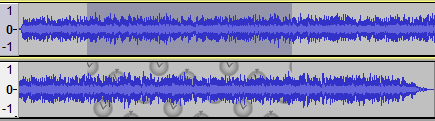
\includegraphics[width=11.509cm,height=3.201cm]{TourGuide-img016.png} 

A pair of Sync-Locked mono tracks: selection extends automatically to the second track

\subsubsection[Sync{}-Lock]{\href{https://manual.audacityteam.org/man/sync_locked_track_groups.html}{\textcolor[rgb]{0.3529412,0.21176471,0.5882353}{Sync-Lock}}}
{\color{black}
When you have a mix (several tracks above each other which play together) and everything is nicely lined up, an edit in
one track such as cutting a piece of audio can cause the mix to no longer to play in sync. To keep tracks aligned
despite cutting, pasting or shifting audio, use Sync-Lock Tracks.}

\subsubsection[Labels]{\href{https://manual.audacityteam.org/man/label_tracks.html}{\textcolor[rgb]{0.3529412,0.21176471,0.5882353}{Labels}}}
{\color{black}
Use a Label Track to mark or annotate audio. In conjunction with Sync-Lock you can keep the labels and audio in step.}

\subsubsection[Undo and
Redo]{\href{https://manual.audacityteam.org/man/undo_redo_and_history.html}{\textcolor[rgb]{0.3529412,0.21176471,0.5882353}{Undo
and Redo}}}
\textcolor{black}{These are most useful when working with effects. After you have applied an effect you might change
your mind. The~Undo~button or menu item~}\textbf{\textcolor{black}{Edit {\textgreater} Undo}}\textcolor{black}{~will
let you undo the change.
The~}\href{https://manual.audacityteam.org/man/undo_redo_and_history.html#history}{\textbf{\textcolor[rgb]{0.3529412,0.21176471,0.5882353}{History}}}\textcolor{black}{~menu
item lets you look further back in time and undo more changes in one step.}

\subsubsection[Truncate
Silence]{\href{https://manual.audacityteam.org/man/truncate_silence.html}{\textcolor[rgb]{0.3529412,0.21176471,0.5882353}{Truncate
Silence}}}
{\color{black}
A convenient effect to apply to recordings of interviews and speeches that removes long silences. You can tell it what
to count as a long silence, the loudness level and duration, and how much of each long silence to remove.}

\subsubsection[Snap
To]{\href{https://manual.audacityteam.org/man/selection_toolbar.html\#snap}{\textcolor[rgb]{0.3529412,0.21176471,0.5882353}{Snap
To}}}
{\color{black}
When making selections it sometimes is helpful for the selection boundaries to be automatically moved to the nearest
second (or some other unit of time measurement). If you `snap-to' seconds your selections will always be whole numbers
of seconds - you can't select half a second of sound for example. Set the time format to seconds or frames or whatever
unit of time you want to snap to as well as enabling snap-to.}

\subsubsection[Effects
Plug{}-ins]{\href{https://manual.audacityteam.org/man/customization.html\#plug-ins}{\textcolor[rgb]{0.3529412,0.21176471,0.5882353}{Effects
Plug-ins}}}
\textcolor{black}{You can add to the effects available in Audacity using plug-ins. Some of these have very nice looking
interfaces with graphs and buttons and provide similar effects with different features, or effects that Audacity does
not ship with. There are several types of plug-in.
The~}\href{https://manual.audacityteam.org/man/customization.html\#plug-ins}{\textbf{\textcolor[rgb]{0.3529412,0.21176471,0.5882353}{Nyquist}}}\textcolor{black}{~type
of plug-in, for example, is Audacity's own plug-in format. Nyquist plug-ins can be made just by writing text in a file,
so contributors to Audacity often use this format to create new effects. Thoroughly tested plug-ins are available
from~}\href{https://wiki.audacityteam.org/wiki/Download_Nyquist_Plug-ins}{\textit{\textcolor[rgb]{0.2,0.4,0.73333335}{Download
Nyquist Plug-ins}}}\textcolor{black}{. Experimental plug-ins, such as those for the hard task of removing pops, clicks
and {\textquotedbl}ess{\textquotedbl} sounds from a voice recording, can be found on
the~}\href{https://forum.audacityteam.org/viewforum.php?f=39}{\textit{\textcolor[rgb]{0.2,0.4,0.73333335}{Nyquist board
on Audacity Forum}}}\textcolor{black}{.}

\subsubsection[Multi{}-Clip]{\href{https://manual.audacityteam.org/man/audacity_tracks_and_clips.html}{\textcolor[rgb]{0.3529412,0.21176471,0.5882353}{Multi-Clip}}}
\textcolor{black}{Many people have a single piece of audio on each audio track. However, you can have multiple pieces of
non-overlapping audio on the same track. These are called clips. Clips can be created
with~}\href{https://manual.audacityteam.org/man/audacity_tracks_and_clips.html#split}{\textbf{\textcolor[rgb]{0.3529412,0.21176471,0.5882353}{Split}}}\textcolor{black}{~and
joined back together by clicking on the dark line boundary between clips. If you click
the~}\href{https://manual.audacityteam.org/man/tools_toolbar.html#timeshift}{\textbf{\textcolor[rgb]{0.3529412,0.21176471,0.5882353}{Time
Shift Tool}}}\textcolor{black}{~you can drag clips around to different positions on the track, or drag them to
different tracks.}
\end{document}
